\olchapter{sfr}{arith}{Arithmetization}

\begin{editorial}
The material in this chapter presents the construction of the number
systems in na\"ive set theory. It is taken from Tim Button's Open Set
Theory text.
\end{editorial}



\olfileid{sfr}{arith}{int}
\olsection{From $\Nat$ to $\Int$}

Here are two basic realisations:
	\begin{enumerate}
		\item Every integer can be written in the form $n - m$, with $n, m \in\Nat$.
		\item The information encoded in an expression $n - m$ can equally be encoded by an ordered pair $\tuple{n, m}$.
	\end{enumerate}
We already know that the ordered pairs of natural numbers are the !!{element}s of $\Nat^2$. And we are assuming that we understand $\Nat$. So here is a na\"{i}ve suggestion, based on the two realisations we have had: \emph{let's treat integers as ordered pairs of natural numbers}.

In fact, this suggestion is too na\"{i}ve. Obviously we want it to be the case that $0- 2 = 4 - 6$. But evidently $\tuple{0, 2 }\neq \tuple{4, 6}$. So we cannot simply say that $\Nat^2$ is the set of integers. 

Generalising from the preceding problem, what we want is the following:
	$$a - b = c - d \text{ iff }a + d = c + b$$
(It should be obvious that this is how integers are \emph{meant} to behave: just add $b$ and $d$ to both sides.) And the easy way to guarantee this behaviour is just to define an equivalence relation between ordered pairs, $\Intequiv$, as follows:
$$\tuple{ a, b } \Intequiv \tuple{c, d}\text{ iff }a + d = c + b$$  
We now have to show that this is an equivalence relation.
\begin{prop} $\Intequiv$ is an equivalence relation.
\end{prop}
	\begin{proof}
	We must show that $\Intequiv$ is reflexive, symmetric, and transitive. 
	
	\emph{Reflexivity:} Evidently $\tuple{a, b} \Intequiv \tuple{a, b}$, since $a + b = b + a$.
	
	\emph{Symmetry:} Suppose $\tuple{a, b} \Intequiv \tuple{c, d}$, so $a + d = c + b$. Then $c + b = a + d$, so that $\tuple{c, d} \Intequiv \tuple{a, b}$.
	
	\emph{Transitivity:} Suppose $\tuple{a, b} \Intequiv \tuple{c, d}\Intequiv \tuple{m, n}$. So $a + d = c + b$ and $c + n = m + d$. So $a + d + c + n = c + b + m + d$, and so $a + n = m + b$. Hence $\tuple{a, b } \Intequiv \tuple{m, n}$.		
\end{proof}

Now we can use this equivalence relation to take equivalence classes:

\begin{defn}
		The integers are the equivalence classes, under $\Intequiv$, of  ordered pairs of natural numbers; that is, $\Int = \equivclass{\Nat^2}{\Intequiv}$.
\end{defn}

Now, one might have plenty of different \emph{philosophical} reactions to this stipulative definition. Before we consider those reactions, though, it is worth continuing with some of the technicalities. 

Having said what the integers are, we shall need to define basic functions and relations on them. Let's write $\equivrep{m, n}{\Intequiv}$ for the equivalence class under $\Intequiv$ with $\tuple{m, n}$ as !!a{element}.\footnote{Note: using the notation introduced in \olref[sfr][rel][eqv]{def:equivalenceclass}, we would have written $\equivrep{\tuple{m,n}}{\Intequiv}$ for the same thing. But that's just a bit harder to read.} That is: 
	$$\equivrep{m, n}{\Intequiv} = \Setabs{\tuple{a, b} \in \Nat^2}{\tuple{a, b}\Intequiv \tuple{m, n}}$$
So now we offer some definitions:
	\begin{align*}
		\equivrep{a, b}{\Intequiv} + \equivrep{c, d}{\Intequiv} &= \equivrep{a + c, b + d}{\Intequiv}\\
		\equivrep{a, b}{\Intequiv} \times \equivrep{c, d}{\Intequiv} &= \equivrep{a c + b  d, a  d + b c}{\Intequiv}\\
		\equivrep{a, b}{\Intequiv} \leq \equivrep{c, d}{\Intequiv} &\text{ iff }a + d \leq b + c
	\end{align*}	
(As is common, I'm using `$ab$' stand for `$(a \times b)$', just to make the axioms easier to read.) Now, we need to make sure that these definitions behave as they \emph{ought} to. Spelling out what this means, and checking it through, is rather laborious; we relegate the details to \olref[check]{sec}. But the short point is: everything works! 

One final thing remains. We have constructed the integers using
natural numbers. But this will mean that the natural numbers \emph{are
not themselves integers}. We will return to the philosophical
significance of this in \olref[ref]{sec}. On a purely technical front,
though, we will need some way to be able to treat natural numbers
\emph{as} integers. The idea is quite easy: for each $n \in \Nat$, we
just stipulate that $n_\Int = \equivrep{n, 0}{\Intequiv}$. We need to
confirm that this definition is well-behaved, i.e., that for any $m, n
\in \Nat$
\begin{align*}
	(m + n)_\Int &= m_\Int + n_\Int\\
	(m \times n)_\Int &= m_\Int \times n_\Int\\
	m \leq n &\liff m_\Int \leq n_\Int
\end{align*}
But this is all pretty straightforward. For example, to show that the
second of these obtains, we can simply help ourselves to the behaviour
of the natural numbers and reason as follows:


	\begin{align*}

		(m \times n)_\Int  &= \equivrep{m \times n, 0}{\Intequiv} \\
		&= \equivrep{m \times n + 0 \times 0, m \times 0 + 0 \times n}{\Intequiv} \\
		&= \equivrep{m, 0}{\Intequiv} \times \equivrep{n, 0}{\Intequiv} \\
		&= m_\Int \times n_\Int
	\end{align*}

We leave it as an exercise to confirm that the other two conditions hold.
\begin{prob}
	Show that $(m + n)_\Int = m_\Int + n_\Int$ and $m \leq n \liff m_\Int \leq n_\Int$, for any $m, n \in \Nat$.
\end{prob}



\olfileid{sfr}{arith}{rat}
\olsection{From $\Int$ to $\Rat$}

We just saw how to construct the integers from the natural numbers,
using some na\"{i}ve set theory. We shall now see how to construct the
rationals from the integers in a very similar way. Our initial
realisations are:
\begin{enumerate}
	\item Every rational can be written in the form $\nicefrac{i}{j}$,
	where both $i$ and $j$ are integers but $j$ is non-zero.
	\item The information encoded in an expression $\nicefrac{i}{j}$
	can equally be encoded in an ordered pair $\tuple{ i, j}$.
\end{enumerate}
The obvious approach would be to think of the rationals \emph{as}
ordered pairs drawn from $\Int \times (\Int \setminus \{0_\Int\})$. As
before, though, that would be a bit too na\"ive, since we want
$\nicefrac{3}{2} = \nicefrac{6}{4}$, but $\tuple{ 3, 2}\neq \tuple{ 6,
4}$. More generally, we will want the following:
\[
	\nicefrac{a}{b} = \nicefrac{c}{d} \text{ iff } a \times d = b \times c
\]
To get this, we define an {equivalence relation} on  $\Int \times
(\Int \setminus \{0_\Int\})$ thus:
\[
	\tuple{ a, b }\Ratequiv \tuple{ c, d} \text{ iff }a \times d = b \times c
\]
We must check that this is an equivalence relation. This is very much
like the case of $\Intequiv$, and we will leave it as an exercise. 
\begin{prob}
Show that $\Ratequiv$ is an equivalence relation.
\end{prob}
But it allows us to say:
\begin{defn}
The rationals are the equivalence classes, under $\Ratequiv$, of pairs
of integers (whose second element is non-zero). That is, $\Rat =
\equivclass{(\Int \times (\Int\setminus \{0_\Int\}))}{\Ratequiv}$.
\end{defn}

As with the integers, we also want to define some basic operations.
Where $\equivrep{i,j}{\Ratequiv}$ is the equivalence class under
$\Ratequiv$ with $\tuple{i, j}$ as !!a{element}, we say:
\begin{align*}
	\equivrep{a, b}{\Ratequiv} + \equivrep{c, d}{\Ratequiv} &= \equivrep{ad + bc,  bd}{\Ratequiv}\\
	\equivrep{a, b}{\Ratequiv} \times \equivrep{c, d}{\Ratequiv} &= \equivrep{a  c, b d}{\Ratequiv}.
\intertext{To define $r \leq s$ on these rationals, we use the fact that 
$r \le s$ iff $s - r$ is not negative, i.e., $r - s$ can be written as 
$\nicefrac{i}{j}$ with $i$ non-negative and $j$~positive:}
	\equivrep{a, b}{\Ratequiv} \leq \equivrep{c, d}{\Ratequiv} &\text{ iff }
	\equivrep{c, d}{\Ratequiv} - \equivrep{a, b}{\Ratequiv} = 
	\equivrep{i_\Int, j_\Int}{\Ratequiv}
\end{align*}
for some $i \in \Nat$ and $0 \neq j \in \Nat$.

We then need to check that these definitions behave as they
\emph{ought} to; and we relegate this to \olref[check]{sec}. But they
indeed do!{} Finally, we want some way to treat integers \emph{as}
rationals; so for each $i \in \Int$, we stipulate that $i_\Rat =
\equivrep{i, 1_\Int}{\Ratequiv}$. Again, we check that all of this
behaves correctly in \olref[check]{sec}.

\begin{prob}
Show that $(i + j)_\Rat = i_\Rat+ j_\Rat$ and $(i \times j)_\Rat =
i_\Rat \times j_\Rat$ and $i \leq j \liff i_\Rat \leq j_\Rat$, for any
$i, j \in \Int$.
\end{prob}




\olfileid{sfr}{arith}{real}
\olsection{The Real Line}

The next step is to show how to construct the reals from the
rationals. Before that, we need to understand what is
\emph{distinctive} about the reals. 

The reals behave very much like the rationals. (Technically, both are
examples of \emph{ordered fields}; for the definition of this, see
\olref[check]{orderedfield}.) Now, if you worked through the exercises
to \olref[sfr][siz][]{chap}, you will know that there are strictly
more reals than rationals, i.e., that $\cardless{\Rat}{\Real}$. This
was first proved by Cantor. But it's been known for about two and a
half millennia that there are irrational numbers, i.e., reals which
are not rational. Indeed:

\begin{thm}\ollabel{root2irrational}
$\sqrt{2}$ is not rational, i.e., $\sqrt{2} \notin \Rat$
\end{thm}

\begin{proof}
Suppose, for reductio, that $\sqrt{2}$ is rational. So $\sqrt{2} =
\nicefrac{m}{n}$ for some natural numbers $m$ and $n$. Indeed, we can
choose $m$ and $n$ so that the fraction cannot be reduced any further.
Re-organising, $m^{2} = 2n^{2}$. From here, we can complete the proof
in two ways:

\emph{First, geometrically} (following Tennenbaum).\footnote{This
proof is reported by \cite{Conway2006}.} Consider these squares:
\begin{center}	
	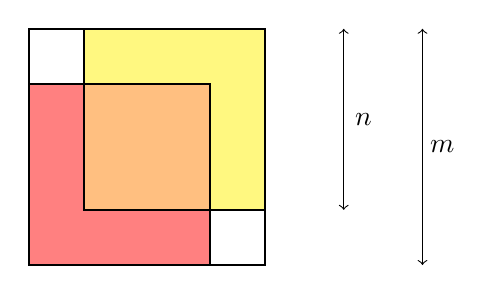
\begin{tikzpicture}
		\draw[thick] (0,0) rectangle (3,3);
		\draw[thick, fill=red!50] (0,0) rectangle (2.3,2.3);
		\draw[thick, fill=yellow!50] (0.7,0.7) rectangle (3, 3);
		\draw[thick, fill=orange!50] (0.7,0.7) rectangle (2.3, 2.3);
		\draw[<->] (4, 0.7)--(4, 3);
		\node at (4.25, 1.85) (n) {$n$};
		\draw[<->] (5, 0)--(5, 3);
		\node at (5.25, 1.5) (m) {$m$};
	\end{tikzpicture}
\end{center}
Since $m^2 = 2n^2$, the region where the two squares of side $n$
overlap has the same area as the region which neither of the two
squares cover; i.e., the area of the orange square equals the sum of
the area of the two unshaded squares. So where the orange square has
side $p$, and each unshaded square has side $q$, $p^2 = 2q^2$. But now
$\sqrt{2} = \nicefrac{p}{q}$, with $p < m$ and $q < n$ and $p, q \in
\Nat$. This contradicts the fact that $m$ and $n$ were chosen to be as
small as possible.
		
\emph{Second, formally.} Since $m^{2} = 2n^{2}$, it follows that $m$
is even. (It is easy to show that, if $x$ is odd, then $x^2$ is odd.)
So $m = 2r$, for some $r \in \Nat$. Rearranging, $2r^2 = n^2$, 
		
		
		
		
		
so $n$ is also even. So both $m$ and $n$ are even, and hence the
fraction $\nicefrac{m}{n}$ \emph{can} be reduced further.
Contradiction!
\end{proof}

In passing, this diagrammatic proof allows us to revisit the material from \olref[his][set][mythology]{sec}. Tennenbaum (1927--2006) was a thoroughly modern mathematician; but the proof is undeniably lovely, completely rigorous, and appeals to geometric intuition!

In any case: the reals are ``more expansive'' than the rationals. In some sense, there are ``gaps'' in the rationals, and these are filled by the reals. Weierstrass realised that this describes a single property of the real numbers, which distinguishes them from the rationals, namely the Completeness Property: \emph{Every non-empty set of real numbers with an upper bound has a least upper bound.} 

It is easy to see that the rationals do not have the Completeness Property. For example, consider the set of rationals less than $\sqrt{2}$, i.e.:
\[
	\Setabs{p \in \Rat}{p^2 < 2 \text{ or }p < 0}
\]
This has an upper bound in the rationals; its !!{element}s< are all  smaller than $3$, for example. But what is its least upper bound? We want to say `$\sqrt{2}$'; but we have just seen that $\sqrt{2}$ is \emph{not} rational. And there is no \emph{least} rational number greater than $\sqrt{2}$. So the set has an upper bound but no least upper bound. Hence the rationals lack the Completeness Property.

By contrast, the continuum ``morally ought'' to have the Completeness Property. We do not just want $\sqrt{2}$ to be a real number; we want to fill all the ``gaps'' in the rational line. Indeed, we want the continuum itself to have no ``gaps'' in it. That is just what we will get via Completeness.




\olfileid{sfr}{arith}{cuts}
\olsection{From $\Rat$ to $\Real$}

In essence, the Completeness Property shows that any point $\alpha$ of
the real line divides that line into two halves perfectly: those for
which $\alpha$ is the least upper bound, and those for which $\alpha$
is the greatest lower bound. To \emph{construct} the real numbers from
the rational numbers, Dedekind suggested that we simply think of the
reals as the \emph{cuts} that partition the rationals. That is, we
identify $\sqrt{2}$ with the \emph{cut} which separates the rationals
$< \sqrt{2}$ from the rationals $> \sqrt{2}$. 

Let's tidy this up. If we cut the rational numbers into two halves, we
can uniquely identify the partition we made just by considering its
\emph{bottom} half. So, getting precise, we offer the following
definition:

\begin{defn}[Cut] 
A \emph{cut} $\alpha$ is any non-empty proper
initial segment of the rationals with no greatest element. That is,
$\alpha$ is a cut iff:
\begin{enumerate}
	\item \emph{non-empty, proper}: $\emptyset \neq \alpha \subsetneq \Rat$
	\item \emph{initial}: for all $p,q \in \Rat$: if $p < q \in \alpha$ then $p \in \alpha$
	\item \emph{no maximum}: for all $p \in \alpha$ there is a $q \in \alpha$ such that $p < q$ 
\end{enumerate} 
Then $\Real$ is the set of cuts. 
\end{defn}

So now we can say that $\sqrt{2} = \Setabs{p \in \Rat}{p^2 < 2\text{
or }p < 0}$. Of course, we need to check that this \emph{is} a cut,
but we relegate that to \olref[check]{sec}.

As before, having defined some entities, we next need to define basic
functions and relations upon them. We begin with an easy one:
\begin{align*}
	\alpha \leq \beta \text{ iff }\alpha \subseteq \beta
\end{align*}
This definition of an order allows to \emph{state} the central result,
that the set of cuts has the Completeness Property. Spelled out fully,
the statement has this shape. If $S$ is a non-empty set of cuts with
an upper bound, then $S$ has a least upper bound. In more detail: there is a cut, $\lambda$, which is an upper bound for $S$, i.e.\ $(\forall \alpha \in S)\alpha \subseteq
\lambda$, and $\lambda$ is the least such cut, i.e.\ $(\forall \beta \in \Real)((\forall \alpha \in S)\alpha \subseteq \beta \lif \lambda \subseteq \beta)$. Now here is
the proof of the result:

\begin{thm}\ollabel{realcompleteness}
The set of cuts has the Completeness Property. 
\end{thm}

\begin{proof}
Let $S$ be any non-empty set of cuts with an upper bound. Let $\lambda
= \bigcup S$. 

We first claim that $\lambda$ is a cut:
\begin{enumerate}
\item Since $S$ has an upper bound, at least one cut is in $S$, so
$\emptyset \neq \lambda$. Since $S$ is a set of cuts, $\lambda
\subseteq \Rat$. Since $S$ has an upper bound, some $p \in \Rat$ is
absent from every cut $\alpha \in S$. So $p\notin \lambda$, and hence
$\lambda \subsetneq \Rat$.
\item Suppose $p < q \in \lambda$. So there is some $\alpha \in S$
such that $q \in \alpha$. Since $\alpha$ is a cut, $p \in \alpha$. So
$p \in \lambda$.
\item Suppose $p \in \lambda$. So there is some $\alpha \in S$ such
that $p \in \alpha$. Since $\alpha$ is a cut, there is some $q \in
\alpha$ such that $p < q$. So $q \in \lambda$. 
\end{enumerate}
This proves the claim. Moreover, clearly $(\forall \alpha \in S)\alpha
\subseteq \bigcup S = \lambda$, i.e.\ $\lambda$ is an upper bound on $S$. So now suppose $\beta \in \mathbb{R}$ is also an upper bound, i.e.\ $(\forall \alpha \in S)\alpha \subseteq \beta$. For any $p \in \Rat$, if $p \in \lambda$, then there is $\alpha \in S$ such that $p \in \alpha$, so that $p \in \beta$. Generalizing, $\lambda \subseteq \beta$. So $\lambda$ is the \emph{least} upper bound on $S$.
\end{proof}

So we have a bunch of entities which satisfy the Completeness
Property. And one way to put this is: there are no ``gaps'' in our
cuts. (So: taking further ``cuts'' of reals, rather than rationals,
would yield no interesting new objects.)

Next, we must define some operations on the reals. We start by
embedding the rationals into the reals by stipulating that $p_\Real =
\Setabs{q \in \Rat}{q < p}$ for each $p \in \Rat$. We then define:
\begin{align*}
	\alpha + \beta &= \Setabs{p + q}{p \in \alpha \land q \in \beta}\\

	\alpha \times \beta &= 
	\Setabs{p \times q}{0 \leq p \in \alpha \land 0 \leq q \in \beta} \cup 0^\mathbb{R} & \text{if }\alpha, \beta \geq 0_\Real


\end{align*}
To handle the other multiplication cases, first let: 
\begin{align*}
	-\alpha &= \Setabs{p - q}{p < 0 \land q \notin \alpha}
\end{align*}
and then stipulate:
\begin{align*}
	\alpha \times \beta &\defis 
	\begin{cases}
		\mathord{-}\alpha \times \mathord{-}\beta &\text{if }\alpha < 0_\Real\text{ and }\beta < 0_\Real\\
		\mathord{-}(\mathord{-}\alpha \times \beta) &\text{if }\alpha < 0_\Real \text{ and }\beta > 0_\Real\\
		\mathord{-}(\alpha \times \mathord{-}\beta) &\text{if }\alpha > 0_\Real \text{ and }\beta < 0_\Real
	\end{cases}
\end{align*}
We then need to check that each of these definitions always yields a
cut. And finally, we need to go through an easy (but long-winded)
demonstration that the cuts, so defined, behave exactly as they
should. But we relegate all of this to \olref[check]{sec}.



\olfileid{sfr}{arith}{ref}
\olsection{Some Philosophical Reflections}

So much for the technicalities. But what did they achieve?

Well, pretty uncontestably, they gave us some {lovely} pure mathematics. Moreover,
there were some deep conceptual achievements. It was a profound
insight, to see that the Completeness Property expresses the crucial
difference between the reals and the rationals. Moreover, the explicit
construction of reals, as Dedekind cuts, puts the subject matter of
analysis on a firm footing. We know that the notion of a
\emph{complete ordered field} is coherent, for the cuts form just such
a field. 

For all that, we should air a few reservations about these achievements. 

First, it is not clear that thinking of reals in terms of cuts is any
\emph{more} rigorous than thinking of reals in terms of their familiar
(possibly infinite) decimal expansions. This latter ``construction''
of the reals has some resemblance to the construction of the reals via
Cauchy sequence; but in fact, it was essentially known to
mathematicians from the early 17th century onwards (see
\olref[cauchy]{sec}). The real increase in rigour came from the
realisation that the reals have the Completeness Property; the ability
to construct real numbers as particular sets is perhaps not, by
itself, so very interesting.

It is even less clear that the (much easier) arithmetization of the
integers, or of the rationals, increases rigour in those areas. Here,
it is worth making a simple observation. Having \emph{constructed} the
integers as equivalence classes of ordered pairs of naturals, and then
constructed the rationals as equivalence classes of ordered pairs of
integers, and then constructed the reals as sets of rationals, we
immediately \emph{forget about} the constructions. In particular: no
one would ever want to \emph{invoke} these constructions during a
mathematical proof (excepting, of course, a proof that the
constructions behaved as they were supposed to). It's much easier to
speak about a real, directly, than to speak about some set of sets of
sets of sets of sets of sets of sets of naturals. 













	
It is most doubtful of all that these definitions tell us what the
integers, rationals, or reals \emph{are}, \emph{metaphysically
speaking}. That is, it is doubtful that the reals (say) \emph{are}
certain sets (of sets of sets\ldots). The main barrier to such a view
is that the construction could have been done in many different ways.
In the case of the reals, there are some genuinely interestingly
different constructions (see \olref[cauchy]{sec}). But here is a
really trivial way to obtain some different constructions: as in
\olref[sfr][rel][ref]{sec}, we could have defined ordered pairs
slightly differently; if we had used this alternative notion of an
ordered pair, then our constructions would have worked precisely as
well as they did, but we would have ended up with different objects.
As such, there are many rival set-theoretic constructions of the
integers, the rationals, and the reals. And now it would just be
arbitrary (and embarrassing) to claim that the integers (say) are
\emph{these} sets, rather than \emph{those}. (As in
\olref[sfr][rel][ref]{sec}, this is an instance of an argument made
famous by \citealt{Benacerraf1965}.)

A further point is worth raising: there is something quite \emph{odd}
about our constructions. We started with the natural numbers. We then
construct the integers, and construct ``the $0$ of the integers'',
i.e., $ \equivrep{0,0}{\Intequiv}$. But $0 \neq
\equivrep{0,0}{\Intequiv}$. Indeed,  given our constructions,
\emph{no} natural number is an integer. But that seems extremely
counter-intuitive. Indeed, in \olref[sfr][set][imp]{sec}, we claimed
without much argument that $\Nat \subseteq \Rat$. If the constructions
tell us exactly \emph{what} the numbers are, this claim was trivially
false. 

Standing back, then, where do we get to? Working in a na\"ive set
theory, and helping ourselves to the naturals, we are able to
\emph{treat} integers, rationals, and reals as certain sets. In that
sense, we can \emph{embed} the theories of these entities within a set
theory. But the philosophical import of this embedding is just not
that straightforward. 

Of course, none of this is the last word!{} The point is only this.
Showing that the arithmetization of the reals \emph{is} of deep
philosophical significance would require some additional
\emph{philosophical} argument.







	
\olfileid{sfr}{arith}{check}
\olsection{Ordered Rings and Fields}

Throughout this chapter, we claimed that certain definitions behave
``as they ought''. In this technical appendix, we will spell out what
we mean, and (sketch how to) show that the definitions do behave
``correctly''. 

In \olref[int]{sec}, we defined addition and multiplication on $\Int$.
We want to show that, as defined, they endow $\Int$ with the structure
we ``would want'' it to have. In particular, the structure in question
is that of a commutative ring.

\begin{defn}
	A \emph{commutative ring} is a set $S$, equipped with specific elements $0$ and $1$ and operations $+$ and $\times$, satisfying these eight formulas:
	\begin{align*}
		\emph{Associativity}&&a + (b+ c) & = (a + b) + c \\
		&& (a \times b) \times c & = a \times (b\times c)\\
		\emph{Commutativity}&&a + b &= b+ a  \\
		&&  a \times b&= b\times a\\ 
		\emph{Identities}&&a + 0 &= a \\
		&& a \times 1 &= a\\
		\emph{Additive Inverse}&&(\exists b\in S)0&=a + b\\
		\emph{Distributivity}&&a \times (b+ c ) &= (a \times b) + (a \times c)
	\end{align*}
	Implicitly, these are all bound with universal quantifiers restricted to $S$. And note that the elements $0$ and~$1$ here need not be the natural numbers with the same name.
\end{defn}

So, to check that the integers form a commutative ring, we just need
to check that we meet these eight conditions. None of the conditions
is {difficult} to establish, but this is a bit laborious. For example,
here is how to prove \emph{Associativity}, in the case of addition:

\begin{proof} 
Fix $i, j, k \in \Int$. So there are $a_1, b_1, a_2, b_2, a_3, b_3 \in
\Nat$ such that $i = \equivrep{a_1, b_1}{}$ and $j =
\equivrep{a_2,b_2}{}$ and $k = \equivrep{a_3, b_3}{}$. (For
legibility, we write ``$\equivrep{x, y}{}$'' rather than
``$\equivrep{x, y}{\Intequiv}$''; we'll do this throughout this
section.) Now:
\begin{align*}
	i + (j + k) &= \equivrep{a_1, b_1}{}+(\equivrep{a_2, b_2}{} + \equivrep{a_3, b_3}{}) \\
	&= \equivrep{a_1,  b_1}{} + \equivrep{a_2+a_3, b_2+b_3}{}\\
	&= \equivrep{a_1 + (a_2 + a_3), b_1 + (b_2 + b_3)}{}\\
	&= \equivrep{(a_1 + a_2) + a_3, (b_1 + b_2) + b_3}{}\\
	&= \equivrep{a_1 + a_2, b_1 + b_2}{} + \equivrep{a_3, b_3}{}\\
	&= (\equivrep{a_1, b_1}{} + \equivrep{a_2, b_2}{}) + \equivrep{a_3, b_3}{}\\
	&= (i+j) + k
\end{align*}
helping ourselves freely to the behavior of addition on $\Nat$.
\end{proof}

Equally, here is how to prove \emph{Additive Inverse}:

\begin{proof}
Fix $i \in \Int$, so that $i = \equivrep{a,b}{}$ for some $a,b \in
\Nat$. Let $j = \equivrep{b,a}{} \in \Int$. Helping ourselves to the
behaviour of the naturals, $(a+b) + 0 = 0 + (a+b)$, so that
$\tuple{a+b, b+a} \sim_\Int \tuple{0,0}$ by definition, and hence
$\equivrep{a+b, b+a}{} = \equivrep{0, 0}{} = 0_\Int$. So now $i + j =
\equivrep{a,b}{}+\equivrep{b,a}{}=\equivrep{a+b, b+a}{}= \equivrep{0,
0}{} = 0_\Int$.
\end{proof}

And here is a proof of \emph{Distributivity}:

\begin{proof}
As above, fix $i = \equivrep{a_1, b_1}{}$ and $j =
\equivrep{a_2,b_2}{}$ and $k = \equivrep{a_3, b_3}{}$. Now:
\begin{align*}
	i \times (j + k) 
	&= \equivrep{a_1, b_1}{} \times (\equivrep{a_2,b_2}{} + \equivrep{a_3, b_3}{})\\
	&= \equivrep{a_1, b_1}{} \times \equivrep{a_2 + a_3,b_2+b_3}{}\\
	&= \equivrep{a_1  (a_2 + a_3) + b_1  (b_2+b_3), a_1  (b_2 + b_3) + b_1 (a_2 + a_3)}{}\\
	&= \equivrep{a_1 a_2 + a_1a_3 + b_1 b_2+b_1b_3, a_1 b_2 + a_1b_3 + a_2b_1 + a_3b_1}{}\\		

	&= \equivrep{a_1a_2 + b_1b_2, a_1b_2 + a_2b_1}{} + \equivrep{a_1a_3 + b_1b_3, a_1b_3 + a_3b_1}{}\\
	&= (\equivrep{a_1, b_1}{} \times \equivrep{a_2,b_2}{}) + (\equivrep{a_1, b_1}{} \times  \equivrep{a_3, b_3}{})\\
	&= (i \times j) + (i \times k)
\end{align*}
\end{proof}

We leave it as an exercise to prove the remaining five conditions.
Having done that, we have shown that $\Int$ constitutes a commutative
ring, i.e., that addition and multiplication (as defined) behave as
they should.

\begin{prob}
Prove that $\Int$ is a commutative ring.
\end{prob}

But our task is not over. As well as defining addition and
multiplication over $\Int$, we defined an ordering relation, $\leq$,
and we must check that this behaves as it should. In more detail, we
must show that $\Int$ constitutes an \emph{ordered} ring.\footnote{Recall
	from \olref[sfr][rel][ord]{def:linearorder} that a total order
	is a relation which is reflexive, transitive, anti-symmetric, and connected. 
	In the context of order relations, connectedness is sometimes called
	\emph{trichotomy}, since for any $a$ and $b$ we have $a \leq b \lor a
	= b \lor a \geq b$.} 

\begin{defn}
An \emph{ordered ring} is a commutative ring which is also equipped
with a total order relation, $\leq$, such that:
\begin{align*}
	a \leq b &\lif a + c \leq b + c\\
	(a \leq b \land 0 \leq c) &\lif a \times c \leq b \times c
\end{align*}
\end{defn}

\begin{prob}
Prove that $\Int$ is an ordered ring. 
\end{prob}

As before, it is laborious but routine to show that~$\Int$, as
constructed, is an ordered ring. We will leave that to you.

This takes care of the integers. But now we need to show very similar
things of the rationals. In particular, we now need to show that the
rationals form an ordered \emph{field}, under our given definitions of
$+$, $\times$, and $\leq$:
\begin{defn}\ollabel{orderedfield}
An \emph{ordered field} is an ordered ring which also satisfies:
\begin{align*}
	\emph{Multiplicative Inverse}& & (\forall a \in S \setminus \{0\})(\exists b \in S) a\times b& = 1
\end{align*}
\end{defn}

Once you have shown that $\Int$ constitutes an ordered ring, it is
easy but laborious to show that $\Rat$ constitutes an ordered field.

\begin{prob}
Prove that $\Rat$ is an ordered field.
\end{prob}

Having dealt with the integers and the rationals, it only remains to
deal with the reals. In particular, we need to show that $\Real$
constitutes a \emph{complete} ordered field, i.e., an ordered field
with the Completeness Property. Now, \olref[cuts]{realcompleteness}
established that $\Real$ has the Completeness Property. However, it
remains to run through the (tedious) of checking that $\Real$ is an
ordered field. 

Before tearing off into \emph{that} laborious exercise, we need to
check some more ``immediate'' things. For example, we need a guarantee
that $\alpha + \beta$, as defined, is indeed a \emph{cut}, for any
cuts $\alpha$ and $\beta$. Here is a proof of that fact:

\begin{proof}	
Since $\alpha$ and $\beta$ are both cuts, $\alpha + \beta = \Setabs{p
+ q}{p \in \alpha \land q \in \beta}$ is a non-empty proper subset of
$\Rat$. Now suppose $x < p + q$ for some $p \in \alpha$ and $q \in \beta$.
Then $x - p < q$, so $x - p \in \beta$, and $x = p + (x - p) \in
\alpha + \beta$. So $\alpha + \beta$ is an initial segment of $\Rat$.
Finally, for any $p + q \in \alpha + \beta$, since $\alpha$ and
$\beta$ are both cuts, there are $p_1 \in \alpha$ and $q_1 \in \beta$
such that $p < p_1$ and $q < q_1$; so $p + q < p_1 + q_1 \in \alpha +
\beta$; so $\alpha + \beta$ has no maximum. 
\end{proof}

Similar efforts will allow you to check that $\alpha - \beta$ and
$\alpha \times \beta$ and $\alpha \div \beta$ are cuts (in the last
case, ignoring the case where $\beta$ is the zero-cut). Again, though,
we will simply leave this to you. 

\begin{prob}
Prove that $\Real$ is an ordered field.
\end{prob}

But here is a small loose end to tidy up. In
\olref[cuts]{sec}, we suggest that we can take $\sqrt{2} =
\Setabs{p \in \Rat}{p < 0 \text{ or }p^2 < 2}$. But we do need to show
that this set is a \emph{cut}. Here is a proof of that fact:

\begin{proof}
Clearly this is a nonempty proper initial segment of the rationals; so
it suffices to show that it has no maximum. In particular, it suffices
to show that, where $p$ is a positive rational with $p^2 < 2$ and $q =
\frac{2p+2}{p+2}$, both $p < q$ and $q^2 < 2$. To see that $p < q$,
just note:
\begin{align*}
	p^2 &< 2\\
	p^2 + 2p &< 2 + 2p\\
	p(p + 2) &< 2 + 2p\\
	p &< \tfrac{2+2p}{p+2} = q
\end{align*}
To see that $q^2 < 2$, just note:
\begin{align*}
	p^2 &< 2\\
	2p^2 + 4p + 2 &< p^2 + 4p+ 4\\
	4p^2 + 8p + 4 &< 2(p^2 + 4p + 4)\\
	(2p+2)^2 & <2(p+2)^2\\
	\tfrac{(2p+2)^2}{(p+2)^2} &< 2\\
	q^2 &< 2
\end{align*}
\end{proof}



\olfileid{sfr}{arith}{cauchy}

\olsection{Appendix: the Reals as Cauchy Sequences}

In \olref[cuts]{sec}, we constructed the reals as Dedekind cuts. In
this section, we explain an alternative construction. It builds on
Cauchy's definition of (what we now call) a Cauchy sequence; but the
use of this definition to \emph{construct} the reals is due to other
nineteenth-century authors, notably Weierstrass, Heine, M\'{e}ray and
Cantor. (For a nice history, see \citeauthor{OConnorRobertson:RN}
\citeyear{OConnorRobertson:RN}.)

Before we get to the nineteenth century, it's worth considering Simon
Stevin (1548--1620). In brief, Stevin realised that we can think of
each real in terms of its decimal expansion. Thus even an irrational
number, like $\sqrt{2}$, has a nice decimal expansion, beginning:
\[
	1.41421356237\ldots
\] 
It is very easy to model decimal expansions in set theory: simply
consider them as functions $d \colon \Nat \to \Nat$, where $d(n)$ is
the $n$th decimal place that we are interested in. We will then need a
bit of tweak, to handle the bit of the real number that comes before
the decimal point (here, just $1$). We will also need a further tweak
(an equivalence relation) to guarantee that, for example, $0.999\ldots
= 1$. But it is not difficult to offer a perfectly rigorous
construction of the real numbers, in the manner of Stevin, within set
theory. 

Stevin is not our focus. (For more on Stevin, see
\citealt{KatzKatz2012}.) But here is a closely related thought.
Instead of treating $\sqrt{2}$'s decimal expansion directly, we can
instead consider a  \emph{sequence} of increasingly accurate rational
approximations to $\sqrt{2}$, by considering the increasingly precise
expansions: 
\[
1, 1.4, 1.414, 1.4142, 1.41421,\ldots
\]
The idea that reals can be considered via ``increasingly good
approximations'' provides us with the basis for another sequence of
insights (akin to the realisations that we used when constructing
$\Rat$ from $\Int$, or $\Int$ from $\Nat$). The basic insights are
these:
\begin{enumerate}
	\item Every real can be written as a (perhaps infinite) decimal
	expansion.
	\item The information encoded by a (perhaps infinite) decimal
	expansion can be equally be encoded by a sequence of rational
	numbers.
	\item A sequence of rational numbers can be thought of as a
	function from $\Nat$ to $\Rat$; just let $f(n)$ be the $n$th
	rational in the sequence.
\end{enumerate}
Of course, not just \emph{any} function from $\Nat$ to $\Rat$ will
give us a real number. For instance, consider this function:
\[
	f(n) =\begin{cases}
			1 & \text{if }n\text{ is odd}\\
			0 &\text{if }n\text{ is even}
		\end{cases}
\]
Essentially the worry here is that the sequence $0,1,0,1,0,1,0,\ldots$
doesn't seem to ``hone in'' on any real. So: to ensure that we
consider sequences which do hone in on some real, we need to restrict
our attention to sequences which have some \emph{limit}. 

We have already encountered the idea of a limit, in
\olref[his][set][limits]{sec}. But we cannot use \emph{quite} the same
definition as we used there. The expression ``$(\forall \epsilon>0)$''
there tacitly involved quantification over the real numbers; and we
were considering the limits of functions on the real numbers; so
invoking that definition would be to help ourselves to the real
numbers; and they are exactly what we were aiming to \emph{construct}.
Fortunately, we can work with a closely related idea of a limit. 
\begin{defn}\ollabel{def:CauchySequence}
  A function $f: \Nat \to \Rat$ is a \emph{Cauchy sequence} iff for
  any positive $\epsilon \in \Rat$ we have that $(\exists \ell \in
  \Nat)(\forall m, n > \ell)|f(m) - f(n)| < \epsilon$.
\end{defn}

The general idea of a limit is the same as before: if you want a
certain level of precision (measured by~$\epsilon$), there is a
``region'' to look in (any input greater than~$\ell$). And it is easy
to see that our sequence $1$, $1.4$, $1.414$, $1.4142$,
$1.41421$\ldots has a limit: if you want to approximate $\sqrt{2}$ to
within an error of $\nicefrac{1}{10^{n}}$, then just look to any entry
after the $n$th.

The obvious thought, then, would be to say that a real number just
\emph{is} any Cauchy sequence. But, as in the constructions of $\Int$
and $\Rat$, this would be too na\"{i}ve: for any given real number,
multiple different Cauchy sequences indicate that real number. A
simple way to see this as follows. Given a Cauchy sequence~$f$, define
$g$ to be exactly the same function as~$f$, except that $g(0)\neq
f(0)$. Since the two sequences agree everywhere after the first
number, we will (ultimately) want to say that they have the same
limit, in the sense employed in \olref{def:CauchySequence},
and so should be thought of ``defining'' the same real. So, we should
really think of these Cauchy sequences as the same real number.

Consequently, we again need to define an equivalence relation on the
Cauchy sequences, and identify real numbers with equivalence
relations. First we need the idea of a function which tends to $0$ in
the limit. For any function $h : \Nat \to \Rat$, say that \emph{$h$
tends to $0$} iff for any positive $\epsilon \in \Rat$ we have that
$(\exists \ell \in \Nat)(\forall n > \ell)|h(n)| <
\epsilon$.\footnote{Compare this with the definition of $\lim_{x
\mathord{\rightarrow}\infty}f(x) = 0$ in
\olref[his][set][limits]{sec}.} Further, where $f$ and $g$ are
functions $\Nat \to \Rat$, let $(f-g)(n) = f(n) - g(n)$. Now define:
\[
	f \Realequiv g \text{ iff $(f-g)$ tends to $0$}.
\]
We need to check that $\Realequiv$ is an equivalence relation; and it
is. We can then, if we like, define the reals as the equivalence
classes, under $\Realequiv$, of all Cauchy sequences from $\Nat \to
\Rat$.

\begin{prob}
Let $f(n) = 0$ for every $n$. Let $g(n) = \frac{1}{(n+1)^2}$. Show
that both are Cauchy sequences, and indeed that the limit of both
functions is $0$, so that also $f \sim_\Real g$. 
\end{prob}

Having done this, we shall as usual write $\equivrep{f}{\Realequiv}$
for the equivalence class with $f$ as !!a{element}. However, to keep
things readable, in what follows we will drop the subscript and write
just $\equivrep{f}{}$. We also stipulate that, for each $q \in \Rat$,
we have $q_{\Real} = \equivrep{c_{q}}{}$, where $c_{q}$ is the
constant function $c_q(n) = q$ for all $n \in \Nat$. We then define
basic relations and operations on the reals, e.g.:
\begin{align*}
	\equivrep{f}{} + \equivrep{g}{} &= 	\equivrep{(f + g)}{} \\
	\equivrep{f}{} \times 	\equivrep{g}{} &= \equivrep{(f \times g)}{} 
\end{align*}
where $(f + g)(n) = f(n) + g(n)$ and $(f \times g)(n) = f(n) \times
g(n)$. Of course, we also need to check that each of  $(f + g)$,
$(f-g)$ and $(f\times g)$ are Cauchy sequences when $f$ and $g$ are;
but they are, and we leave this to you.

Finally, we define we a notion of order. Say $\equivrep{f}{}$ is
\emph{positive} iff both $\equivrep{f}{}\neq 0_\Rat$ and $(\exists
\ell \in \Nat)(\forall n > \ell)0 < f(n)$. Then say $\equivrep{f}{} <
\equivrep{g}{}$ iff $\equivrep{(g - f)}{}$ is positive. We have to
check that this is well-defined (i.e., that it does not depend upon
choice of ``representative'' function from the equivalence class). 




But having done this, it is quite easy to show that these yield the
right algebraic properties; that is:
\begin{thm}\ollabel{thm:cauchyorderedfield}
The Cauchy sequences constitute an ordered field.
\end{thm}

\begin{proof}
Exercise. 
\end{proof}

\begin{prob}
Prove that the Cauchy sequences constitute an ordered field.
\end{prob}

It is harder to prove that the reals, so constructed, have the
Completeness Property, so we will give the proof.

\begin{thm}
Every non-empty set of Cauchy sequences with an upper bound has a
least upper bound.
\end{thm}

\begin{proof}[Proof sketch] Let $S$ be any non-empty set of Cauchy
sequences with an upper bound. So there is some $p \in \Rat$ such that
$p_{\Real}$ is an upper bound for $S$. Let $r \in S$; then there is
some $q \in \Rat$ such that $q_{\Real} < r$. So if a least upper bound
on $S$ exists, it is between $q_\Real$ and $p_\Real$ (inclusive). 

We will hone in on the l.u.b., by approaching it simultaneously from
below and above. In particular, we define two functions, $f, g \colon
\Nat \to \Rat$, with the aim that $f$ will hone in on the l.u.b.\ from
above, and $g$ will hone on in it from below. We start by defining:
\begin{align*}
	f(0) &= p \\
	g(0) &= q
\end{align*}
Then, where $a_n = \frac{f(n) + g(n)}{2}$, let:\footnote{This is a
recursive definition. But we have not \emph{yet} given any reason to
think that recursive definitions are ok.}
\begin{align*}
	f(n+1) &=
	\begin{cases}
		a_n &\text{if }(\forall h \in S)\equivrep{h}{} \leq (a_n)_\Real\\
		f(n)&\text{otherwise}
	\end{cases}\\
	g(n+1) &=
	\begin{cases}
		a_n &\text{if }(\exists h \in S)\equivrep{h}{} \geq (a_n)_\Real\\
	 	g(n) &\text{otherwise}
	\end{cases}
\end{align*}
Both $f$ and $g$ are Cauchy sequences. (This can be checked fairly
easily, but we leave it as an exercise.) Note that the function $(f-g)$
tends to $0$, since the difference between $f$ and $g$ halves at each
step. Hence $\equivrep{f}{} = \equivrep{g}{}$. 

We first show that $\equivrep{f}{}$ is an upper bound on $S$, i.e.\ that $(\forall h \in S)\equivrep{h}{} \leq \equivrep{f}{}$.  
(We will invoke \olref{thm:cauchyorderedfield} as we go.) Let $h \in S$ and
suppose, for reductio, that $\equivrep{f}{} < \equivrep{h}{}$, so that
$0_\Real < \equivrep{(h-f)}{}$. Since $f$ is a monotonically
decreasing Cauchy sequence, there is some $n \in \Nat$ such that
$\equivrep{(c_{f(n)} - f)}{} < \equivrep{(h-f)}{}$. So:
\[
	(f(n))_\Real = \equivrep{c_{f(n)}}{} < \equivrep{f}{} + \equivrep{(h-f)}{} = \equivrep{h}{},
\]
contradicting the fact that, by construction, $\equivrep{h}{} \leq (f(n))_\Real$.

We next show that $\equivrep{f}{} = \equivrep{g}{}$ is the \emph{least} upper bound on $S$. So let $j$ be any Cauchy sequence and suppose $\equivrep{j}{} < \equivrep{g}{}$. Reasoning as above (using the fact that $g$ is \emph{increasing}), there is $n \in \Nat$ such that $\equivrep{j}{} < (g(n))_\Real$. But by construction there is $h \in S$ such that $(g(n))_\Real \leq \equivrep{h}{}$, so $\equivrep{j}{} < \equivrep{h}{}$ and therefore $\equivrep{j}{}$ is not an upper bound on $S$.  
\end{proof}



\OLEndChapterHook





